%\begin{figure}[h!]
%    \centering
%    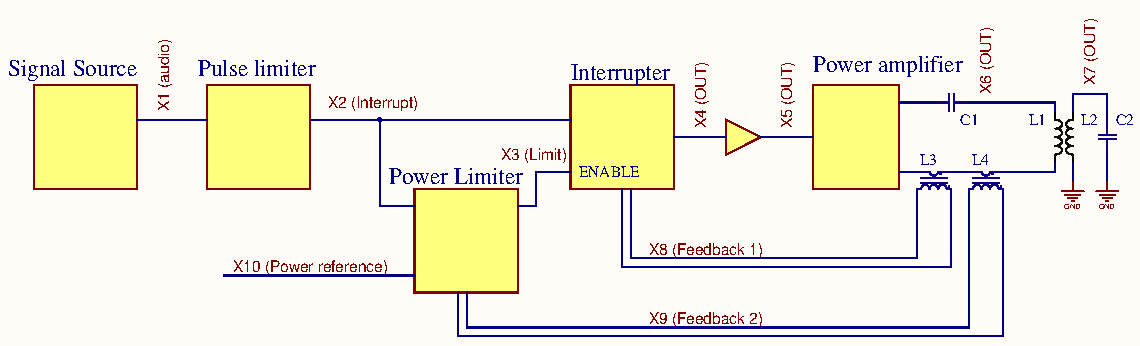
\includegraphics[width=\textwidth]{Skjema/FunksjonsBlokkskjema.pdf}
%    \caption{Block diagram}
%    \label{fig:block}
%\end{figure}

\newpage
\section{Pulse shaper}
The purpose of the pulse shaper is to take the input signal and transform it to be suitable for a DRSSTC, in addition to not letting harmful signals through.

\section{Interrupter}

The interrupter generates the signal which drives the resonant circuit (coil rig) at its resonant frequency $f_0$. As long as the input signal X2 is high the output produces a square wave with fundamental frequency $f_0$. It does this by the means of a positive feedback loop. The feedback signal X8 is retrieved with a sensing transformer around the output wire from the power amplifier, before being clamped, rectified, and schmidt triggered. This results in a cleaned up normalized representation of X8, lets call this signal X8'. The positive flanks of X8' represents when the output current passes zero (this is when we want to switch the polarity of the output). X8' is fed to the output via gates controlled by a latch. One of the outputs is inverted (for push-pull operation). This circuit is shown in \cref{fig:interrupter}, U1A is the latch witch is central to the operation of the interrupter.

\begin{figure}[h!]
    \centering
    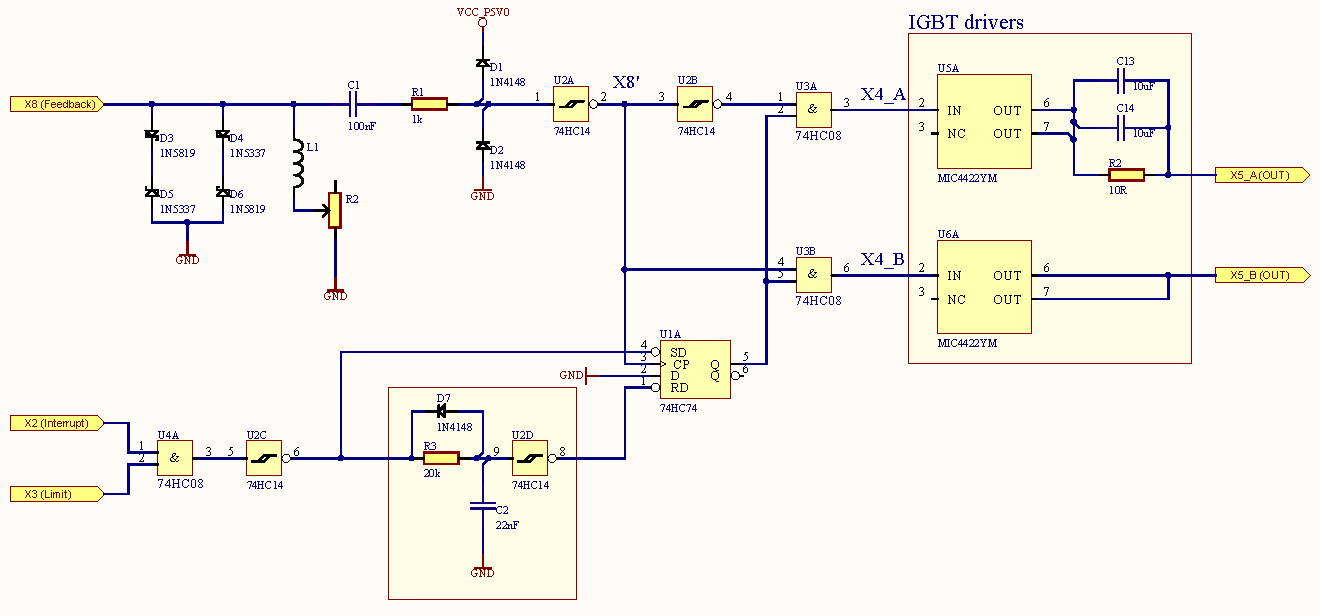
\includegraphics[width=\textwidth]{Skjema/TK514_Interrupter.pdf}
    \caption{Interrupter (TK514)}
    \label{fig:interrupter}
\end{figure}

Initially no current is flowing in the resonant circuit therefore no voltage is present on X8, but because of C1 the the input of U2A is undefined, let us look at the case of the output of U2A being high. Then pin 1 of U1A is low and pin 4 of U1B is high. And the clock input of the latch (U1A) is high. Reset is low. When X2 goes high the SD (Set Data) input of the latch U1A is activated, reset RD goes low, and the output Q goes high. Then X4B goes high and causes a step response in the resonant circuit. The feedback transformer is oriented such that this current direction gives a negative voltage on X8 and thus still low signal on the input of U2A. When the current direction changes the signal on the input of U2A goes from low to high and X4A goes high and X4B goes low. This reverses the voltage on the resonant circuit in phase with the step response and triggers an additional step response in phase with the already ongoing one. This cycle continues until X2 goes low. When X2 goes low SD goes low, but Q is still high until the next negative flank on X8 (inverted through U2A). When D (wich is strapped low) is clocked through the latch. and Q goes low and both X4A and X4B goes low. And no further energy is supplied to the resonant circuit and the step response completes. In the case of the initial value of the output of U2A being low X4\_A would go high first instead of X4\_B and X8 would go high right away. Prompting X4\_A and X4\_B to invert immediately and switch the output while the current is not zero. \todo{Analysere/Diskutere initialverdi på U2A}

\begin{figure}[!ht]
    \centering
    \begin{tikztimingtable}
        X2      & 2L 19H 0.5H 10.5L\\
        X8'     & 2L 1L 19.5{1C} N(A1) 4{1C} 6L\\
        SD      & 2H 19L 0.5L 10.5H\\
        CP      & 2H 1H 24{1C} 5H\\
        D       & 32L\\
        RD      & 2L 28H 2L\\
        Q       & 2L 1H 19H N(B1) 10L\\
        X4\_A   & 2L 1L 19{1C} 10L\\
        X4\_B   & 2L 1H 19{1C} 10L\\
        \extracode
        \tablerules
        \begin{pgfonlayer}{background}
            \draw [help lines] (A1) -- (B1);
        \end{pgfonlayer}
    \end{tikztimingtable}
    \caption{Timing diagram for interrupter}
    \label{fig:tones}
\end{figure}{}

The function of L1 and R2 is to introduce a phase lead on the voltage of X8 in relation of the current on X8. This is to that one can compensate for propagation delays in the circuit and for switching delays in the transistors in the bridge inverter. When the circuit is inductive the voltage will lead the current. By adjusting the value of R2 the relation between the inductance and resistance is changed and thus the phase angle is changed. Thus the time between when the voltage crosses zero and the current crosses zero can be adjusted. This time should theoretically be equal to the time it takes the feedback signal X8 to propagate through the logic and for the IGBT to turn on or off. So that we will switch when the current in the resonant circuit is zero (Zero current switching). This is to reduce energy lost from the resonant circuit and to minimize power burned in the transistors (when switching). From the datasheets we have the propagation delays $t_{pd}$ for the different devices in the propagation path shown in \cref{tab:tpd}. The there are two propagation paths one path contains one scmidth trigger (74HC14) more than the other, also the propagation delay in the mosfet drivers (MIC4422YM) differs for rising and falling outputs. The average propagation delay $t_{pd}$ from the input of U2A to the output of the mosfet drivers is then given by \cref{eq:tpd} and results in $t_{pd} =$ 58 ns typical and 137,5 ns maximum. In addition the delays from hysteresis in U2A $t_hysteresis$ and switching delays in the bridge inverter $t_{sw}$ should be added to the desired phase lead $t_{d}$. Resulting in the desired phase lead $t_{d}$ being given by \cref{eq:td}. The voltage of the feedback signal X8 should have sufficiently high voltage so that delays from hysteresis in U2A is neglible. Delays in the IGBT is read from the datasheet and presented in \cref{tab:tigbt} if we add the delay at 25 $^{\circ}C$ to the nominal $t_d$ and the delay at 150$^{\circ}C$ to the maximum $t_d$, we get a $t_d$ of 141 ns nominal and 258 ns maximum.

Since there are no other resistances in the circuit than R2, as R1 is in series with both a capacitor and the input of the logic gate U2A and can be considered close to infinite in relation to R2, the phase angle is given by \cref{eq:theta}. And thus the desired phase lead is given by \cref{eq:tdl}, and the relation between L and R is given by \cref{eq:lr}. Given a $f_0$ of 110kHz and a desired $t_d$ of 141 ns nominal and 258 ns maximum we get $1,4 \cdot 10^{-7}$ nominal and $2,6 \cdot 10^{-7}$ maximum. The total impedance of L and R should give a sufficently high voltage so that the delay due to hysteresis in U2A is neglible, but not too high voltage for the zener diodes to handle. \todo{Selection of L and R?}

\begin{equation} \label{eq:tpd}
    t_{pd} = t_{pd74HC14} + \frac{t_{pd74HC14}}{2} + t_{pd74HC08} + \frac{t_{pdMIC4422YM Rising}+t_{pdMIC4422YM Falling}}{2}
\end{equation}

\begin{equation} \label{eq:td}
    t_d = t_{hysteresis} + t_{pd} + t_{sw}
\end{equation}

\begin{equation} \label{eq:theta}
    \theta = {tan}^{-1}\frac{X_L}{R} = {tan}^{-1}\frac{\omega L}{R} = {tan}^{-1}\frac{2 \pi f_0 L}{R}
\end{equation}

\begin{equation} \label{eq:tdl}
    t_{d} = \frac{\theta}{\omega} = \frac{\theta}{2 \pi f_0}
\end{equation}

\begin{equation} \label{eq:lr}
    \frac{L}{R} = \frac{{tan}(\theta)}{\omega} = \frac{{tan}(\omega t_{d})}{\omega} = \frac{{tan}(2 \pi f_0 t_{d})}{2 \pi f_0}
\end{equation}

\begin{table}[]
    \centering
    \begin{tabular}{c|c|c}
        Device              & $t_{pd}$ Typ (ns)   & $t_pd$ Max (ns) \\
        74HC14              & 12            & 25\\
        74HC08              & 10            & 20\\
        MIC4422YM Rising    & 20            & 80\\
        MIC4422YM Falling   & 40            & 80
    \end{tabular}
    \caption{Propagation delays for devices}
    \label{tab:tpd}
\end{table}

\begin{table}[]
    \centering
    \begin{tabular}{c|c|c}
                            & $T_J = 25 ^{\circ}C$ & $T_J = 150 ^{\circ}C$ \\
        Turn-On Delay Time (ns)  & 46                & 31    \\
        Turn-Off Delay Time (ns) & 120               & 210
    \end{tabular}
    \caption{Turn on and off delays in the IGBT IRG4PC50WPbF}
    \label{tab:tigbt}
\end{table}

The function of the network connected to the reset (RD) of the latch (U1A) is to reset the latch after a delay in the case that a zero crossing is not detected on X8 after X2 goes low. When X2 goes high the input of U2D goes low immediately due to the capacitor C2 being discharged through D7, but when X2 goes low the capacitor C2 will be charged through R3 and there will be a delay before the latch is reset. The time constant $\tau$ of R3 C2 is 440 $\cdot 10^{-6} s$, the positive going threshold voltage of the schmitt trigger (74HC14) is $T^+ = 2,5V$. We know that a capacitor is charged to $0,5 \cdot VCC$ after $0,7 \tau$, thus the filter R3 C2 together with U2D introduces a delay of 308$\mu s$, or if we have a resonance frequency $f_0$ of 110 Hz a delay of about 34 periods $T = \fraq{1}{f_0}$.

D3-D6 are protection diodes which clamp the feedback signal to safe voltages. The network L1 and R2 introduces a tunable phase lead on the voltage. C1 and R1 is a filter to remove noise. D1 and D2 clamps the voltage to 0-5V.


%%%%%%% Stikkord
%The output of T1 is loaded with a pair of zener diodes with ultrafast diodes to block the slow recovery of the zeners (they are not allowed to be forward biased).  Since the transformer ratio is ~1:1000, by normal transformer action, the current should be 1/1000th of the primary current, and the voltage should be 1000X greater.

%The square wave is also passed through a capacitor to ensure only AC content is passed

%To further protect the logic gate of U1, we have a pair of fast logic diodes to clamp any voltage excursions to the supply rails.

%There are some tricks used to make the JK flip flop (U2) to operate properly in the circuit.  As shown when the interrupter goes HI, CLR\ is LOW.  This puts Q\ in a HI state.  Now, we see that there is a inverter (part of U1) that feeds from the interrupter signal, with its output feeding into an RC circuit and then another inverter.  What this does is delay the HI input to the PRE on the flip flop.  Note that before the PRE is HI, the output from the flip flop is whatever present on CLR\.  If we did not delay the input to PRE, then our interrupter pulse would never be passed along to the gate driver ENABLE (pin 3 on the UCC3732X).  Also note that the flip flop only does its synchronized shut down when PRE is high.  So this leads to choosing what value we want to use for the RC (R9 and C14).  I typically size it so that t=RC=1.5P, where P is the period (in seconds) for 1 RF cycle at the intended operating frequency.  Example, the DRSSTC-1 operates near 60khz, so 1 cycle is 16.67uS, so I would want an RC of about 25uS (whereas I use 22uS).  The important thing is that PRE does not go LOW before the flip flop does its synchronization.  You must allow for at least 1 full cycle of operation after the interrupter has gone LOW for the flip flop to act.  To be on the safe side, you could size the RC to be 3*P.

\newpage
\section{Limiter}

\begin{figure}[h!]
    \centering
    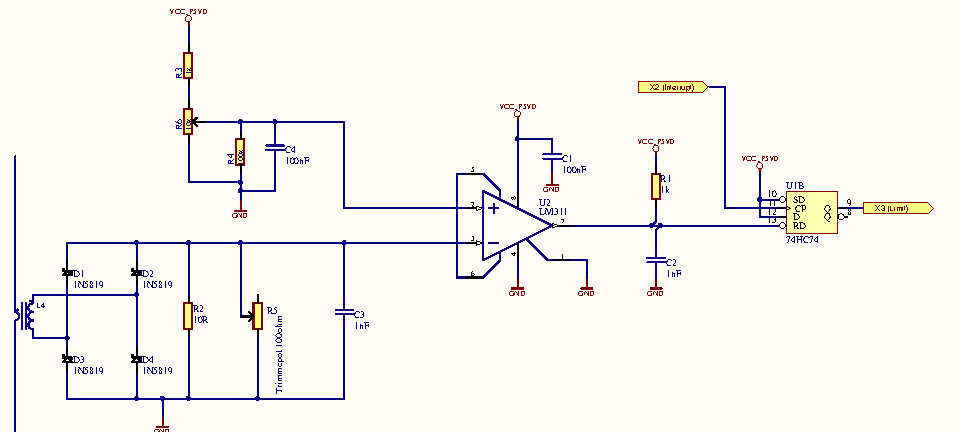
\includegraphics[width=\textwidth]{Skjema/TK513_Limiter.pdf}
    \caption{Limiter}
    \label{fig:my_label}
\end{figure}

The limiter prevents overcurrent in the coil rig. By disabling the interrupter when the peak current rises above a preset level. The diodes D1-D4 is a full bridge rectifier, schottky diodes are used for low propagation delay. The rectifier is loaded with R1, and C1 is a noise filter. The recifier is fed by a feedback transformer connectet to the primary resonant circuit. The rectified signal is fed into a comparator, the other input of the comparator is connected to a potentiometer. R2 is to set the highest level the potentiometer can be set to. R3 is to pull the input of the comparator low in the case that the potentiometer is disconnected.

If the voltage of the rectified feedback signal over R1 is higher than the voltage set by the potentiometer the output of the comparator goes low and resets the latch. The data input of the latch is connected to VCC, on the next positive flank of the interrupt signal X2 the data will be clocked to the output and the output will go high.

The output of the latch is connected to the interrupter. A low signal stops the output of the interrupter. A high signal allows the interrupt signal X2 to control the output.


%%%%%% Stikkord
%The output from the rectifiers is then again loaded down with 100 ohms.  This 100 ohms is to keep the impedance at the comparator (U6) input low, making it somewhat noise immune.  This technique works very well, and without the 100 ohm resistor in place, I find the circuit will falsely trigger on noise.  C15 provides extra noise filtering.

\newpage
\section{Bridge inverter}

\begin{figure}[h!]
    \centering
    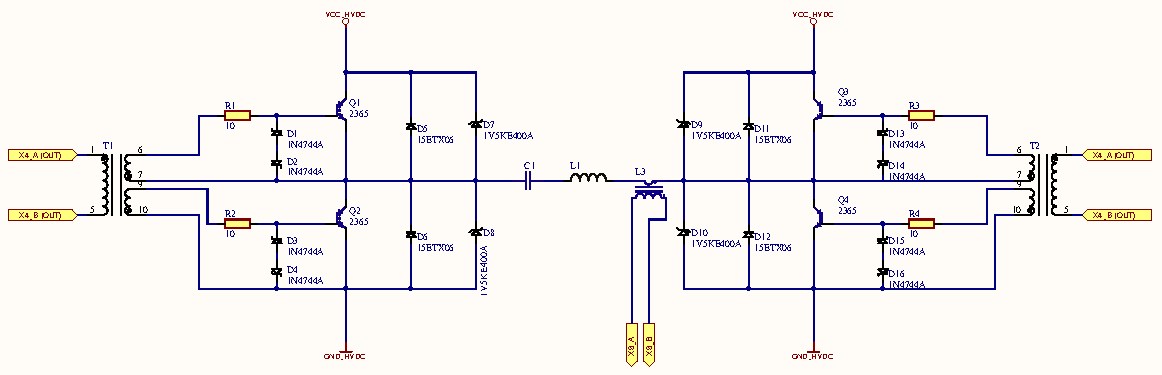
\includegraphics[width=\textwidth]{Skjema/TK531_Utgangstrinn.pdf}
    \caption{Caption}
    \label{fig:tk531}
\end{figure}

The final output stage is a full bridge inverter using IGBTs, IGBTs are chosen over MOSFETs due to IGBTs having lower forward voltage drop at higher voltages and currents. The 1N4744A diodes (15V Zener) is there to clamp the gate voltage to protect the gate of the IGBT from over voltage. The 10 Ohm resistors is to protect from overcurrent. The 1V5KE400A schottky diodes are to protect the IGBTs from reverse voltage transients. The 15ETX06 diodes are there to recycle the leftover energy into the bus capacitors when we have stopped switching, as IGBTs does not conduct reverse current. L3 is the current sense feedback transformer, L1 and C1 is the primary resonant circuit. T1 and T2 are gate drive transformers. The supply voltage VCC\_HVDC is 160VDC.

%%%%%%% Stikkord
%the anti-parallel diodes in the IGBT recycles the leftover energy into the main bus capacitors as the current rings down.

\newpage
\section{Resonant circuit}

\begin{figure}[h!]
    \centering
    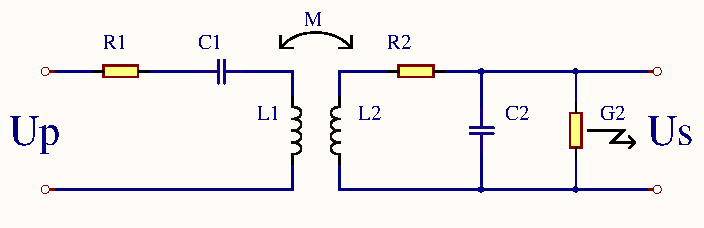
\includegraphics[width=\textwidth]{Skjema/Spolerigg1.pdf}
    \caption{Resonant circuit}
    \label{fig:spolerigg1}
\end{figure}

The resonant circuits step up the voltage from 160VDC to a voltage high enough to create electric arcs. The resonant circuit consists of two parts the primary resonant circuit, and the secondary resonant circuit. When the interrupter first applies a voltage to the primary resonant circuit the circuit repsonds with its step response, this is sinussoidal and whith a frequency equal to the resonant frequency. When the interrupter detects that the current in the primary resonant circuit is zero the polarity switches and we get a new step response added to the already existing one. This continues for several cycles. This current is inductively coupled into the secondary resonant circuit, and when the voltage reaches a high enough level a streamer forms from the top load of the secondary resonant circuit, this drains energy from the secondary circuit, but the streamer continues to grow for a couple of cycles.

%%%%%%%%%%%%% Stikkord
% Løs kobling mellom primær og sekundær for å ikke laste primærkretsen for mye.
% Må tune primær til samme frekvens som sekundær
% Sekundær bestemmer frekvensen.
% Q verdi?

\newpage